\documentclass{article}
\usepackage{graphicx}
\begin{document}
	\section*{Lsg Vorschlag E I Ü10 Maximilian Maag}
	\section*{Aufgabe 10.1}
	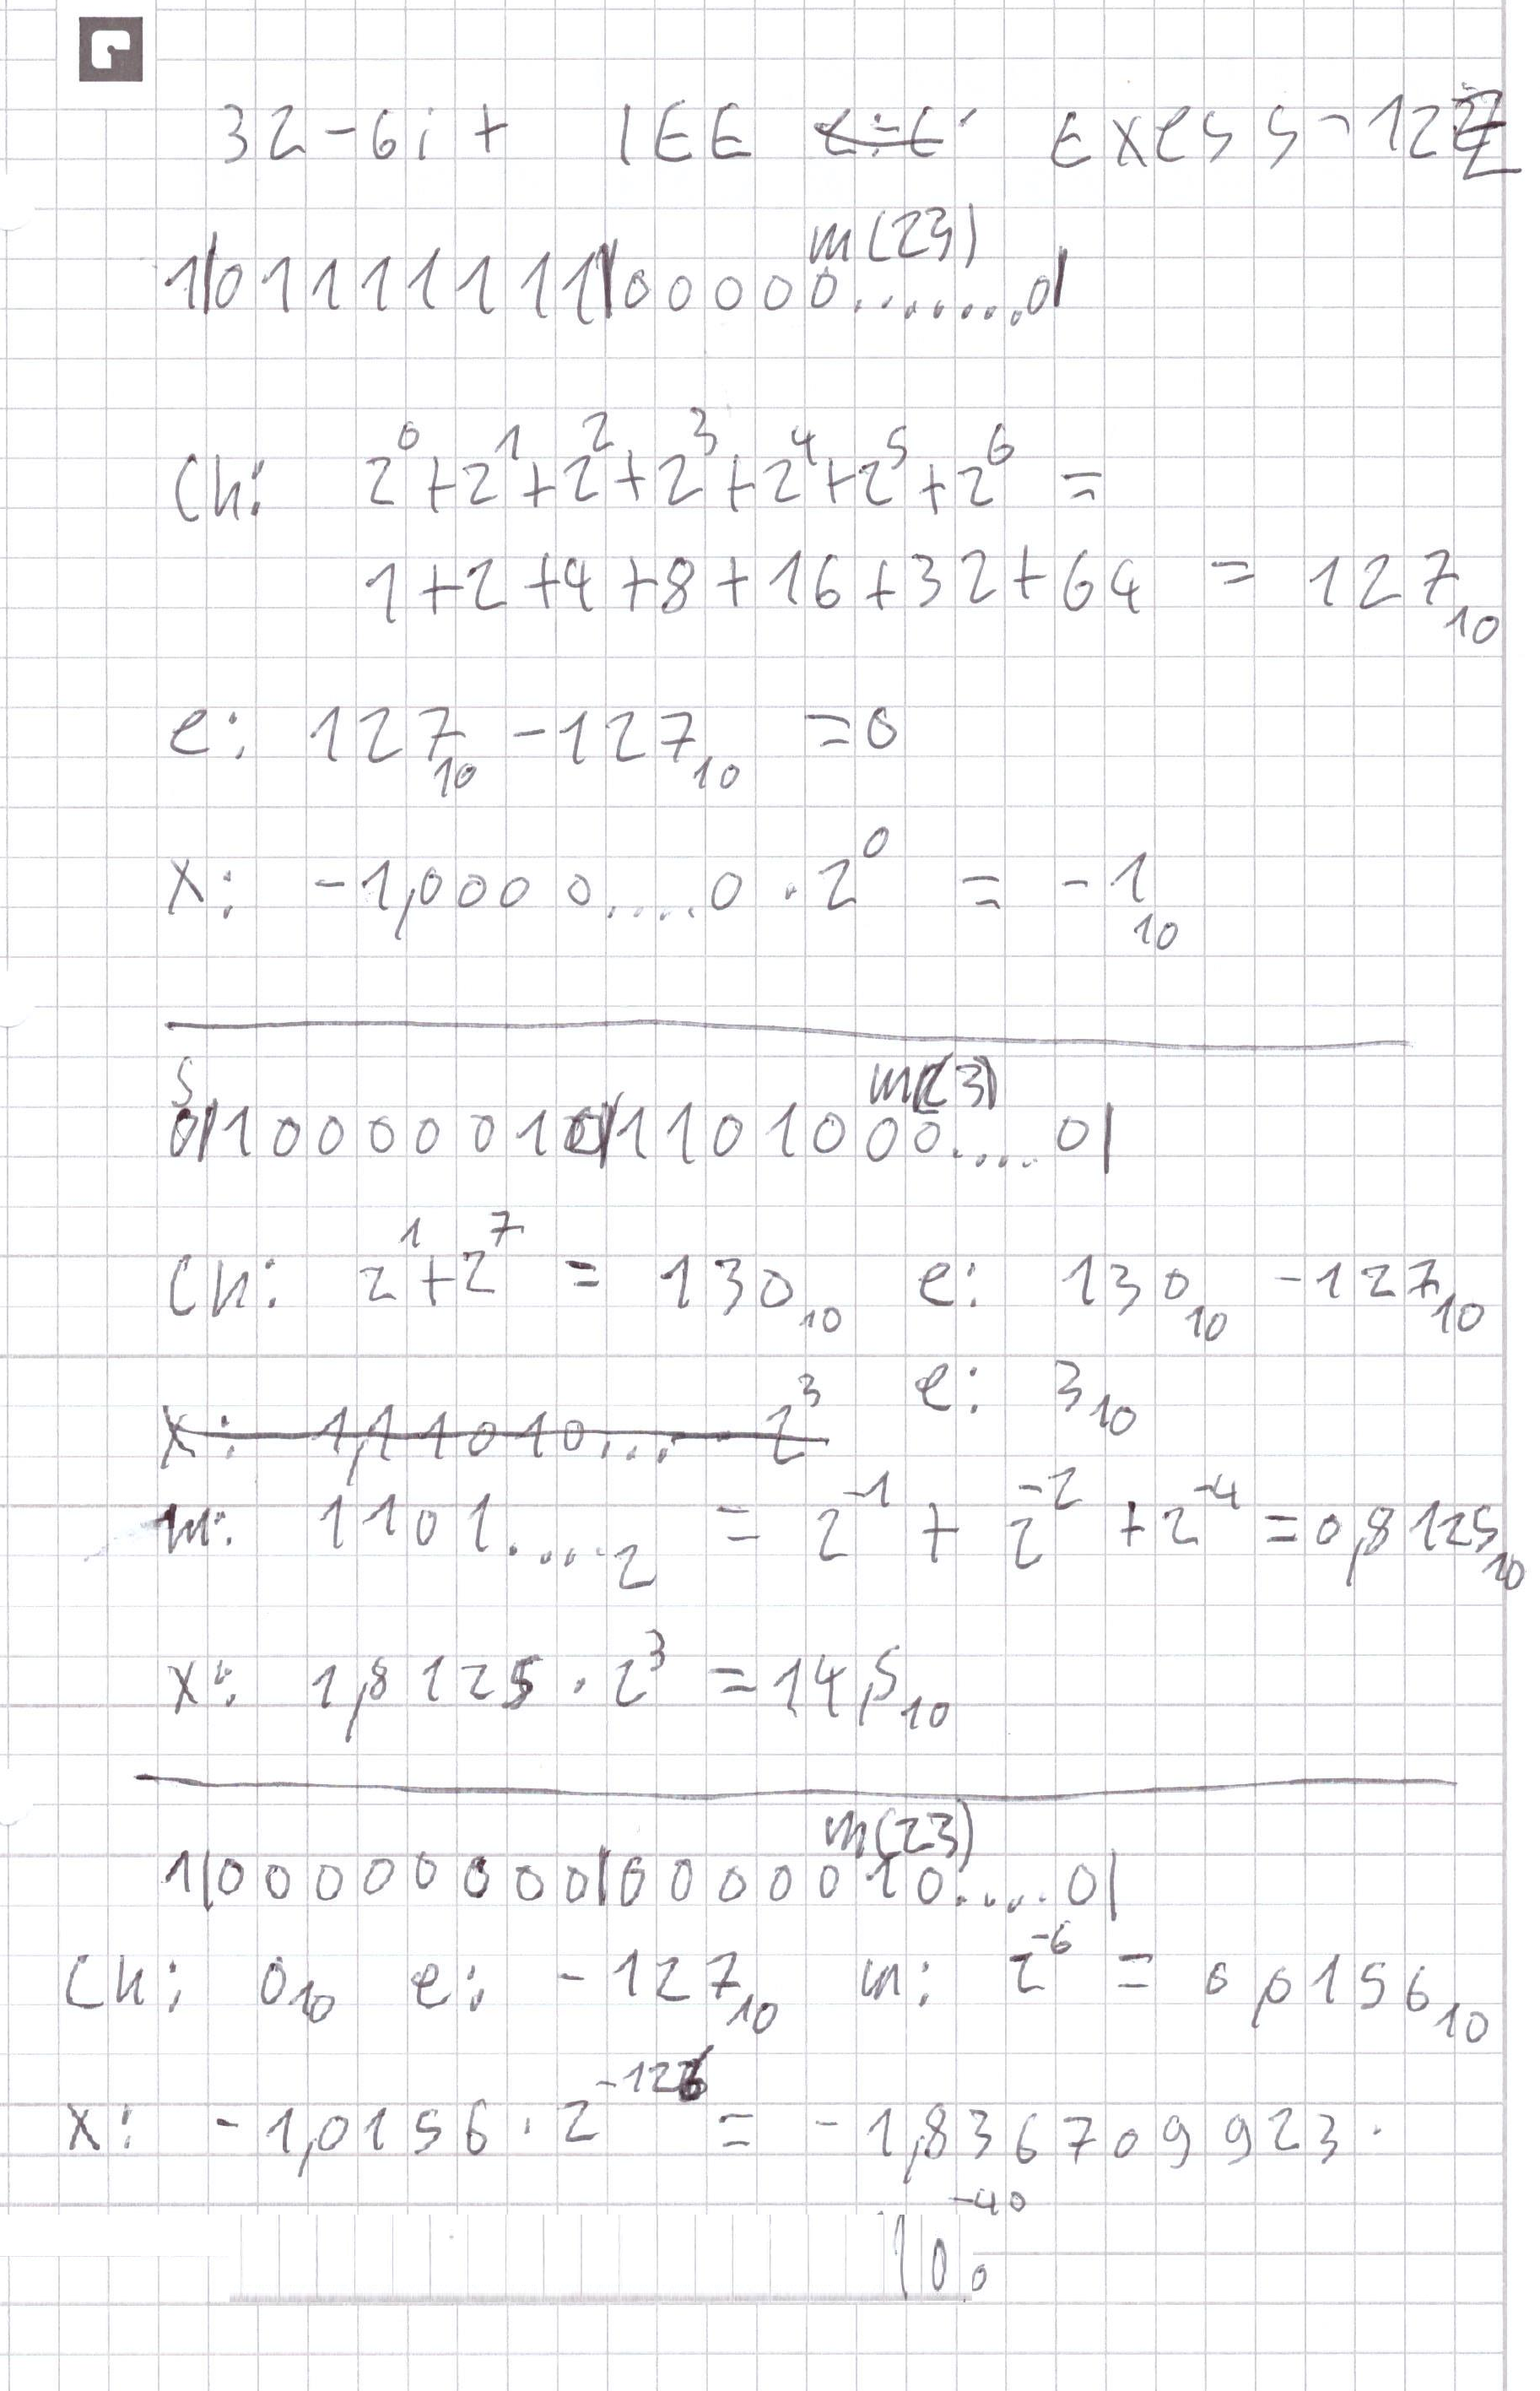
\includegraphics[width=\linewidth, height=\linewidth]{1011} \\
	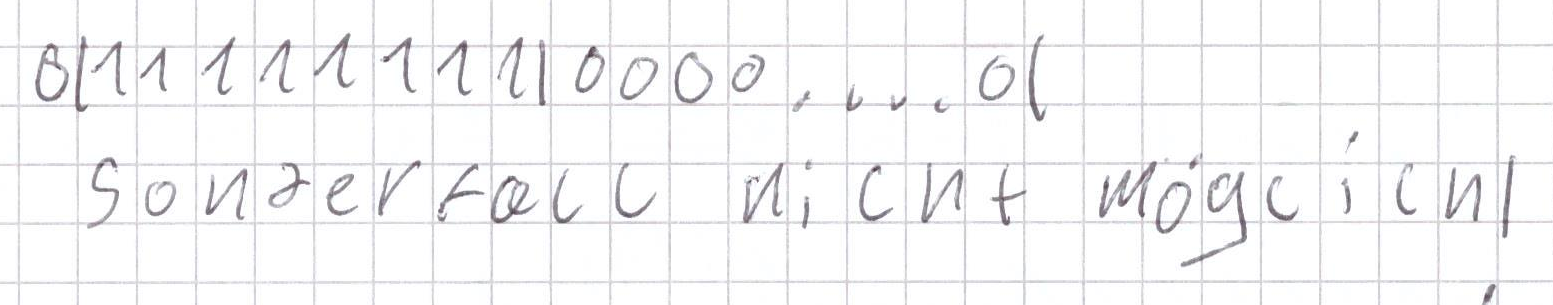
\includegraphics[width=\linewidth]{1012} \\
	Sonderfall Vorzeichen verrät es handelt sich um + $\infty$
	\section*{Aufgabe 10.2}
	\subsection*{a)}
	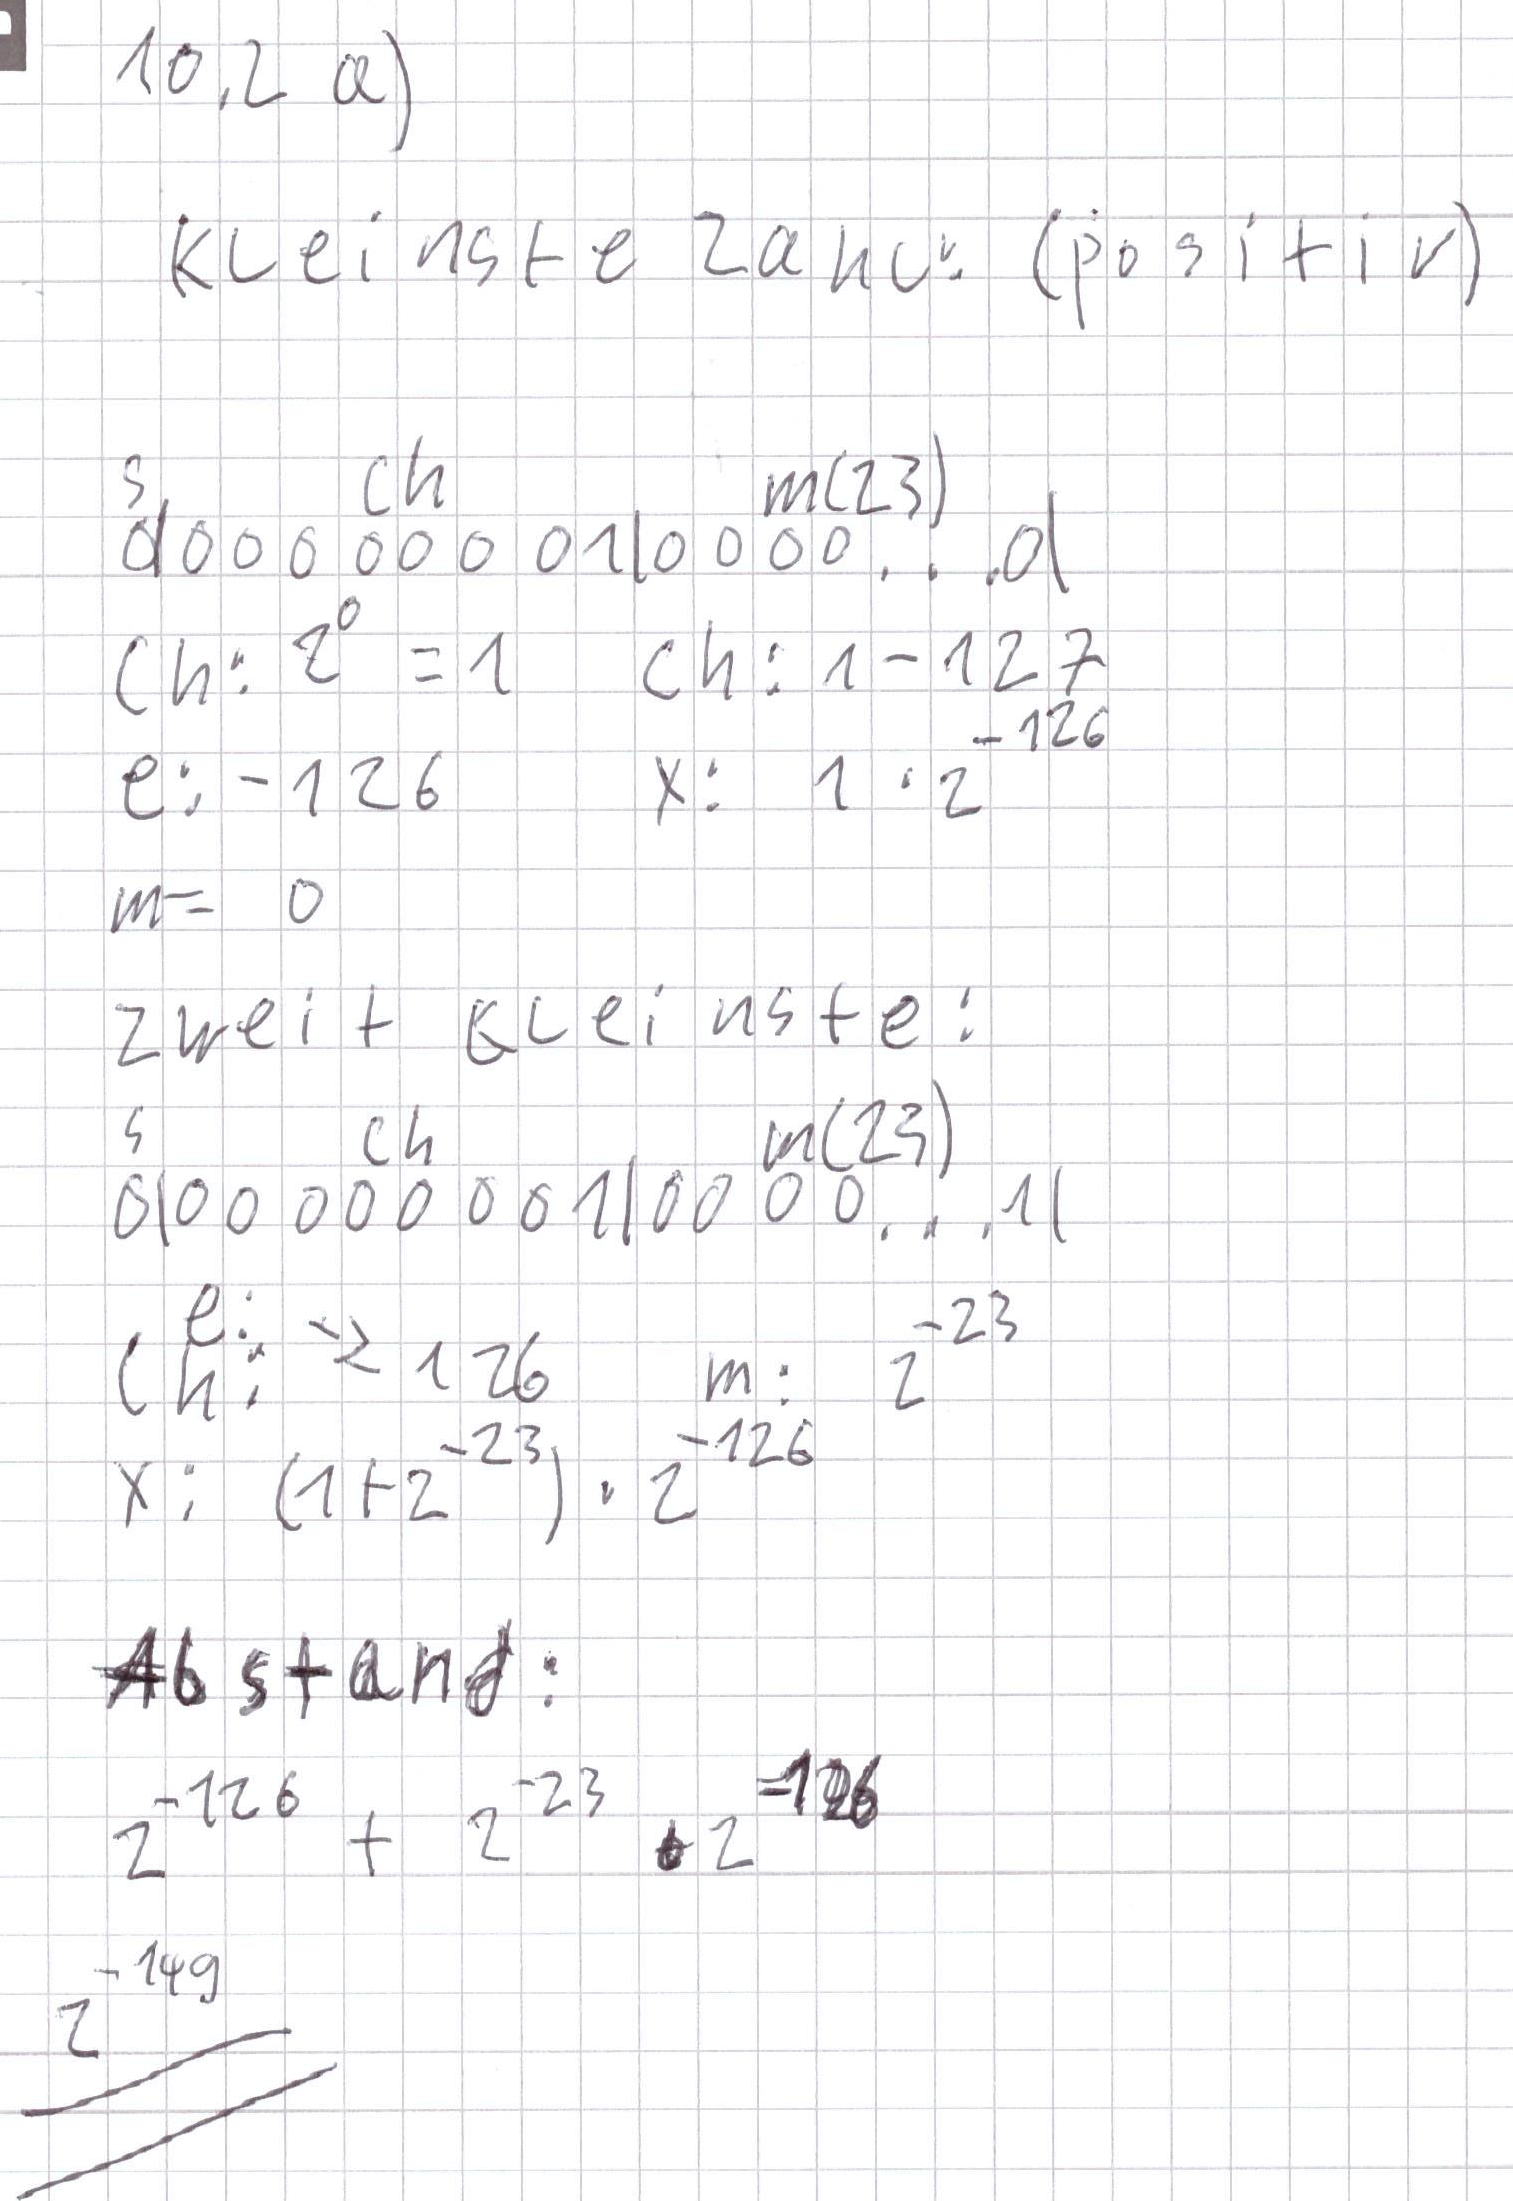
\includegraphics[width=\linewidth]{102a}
	\subsection*{b)}
	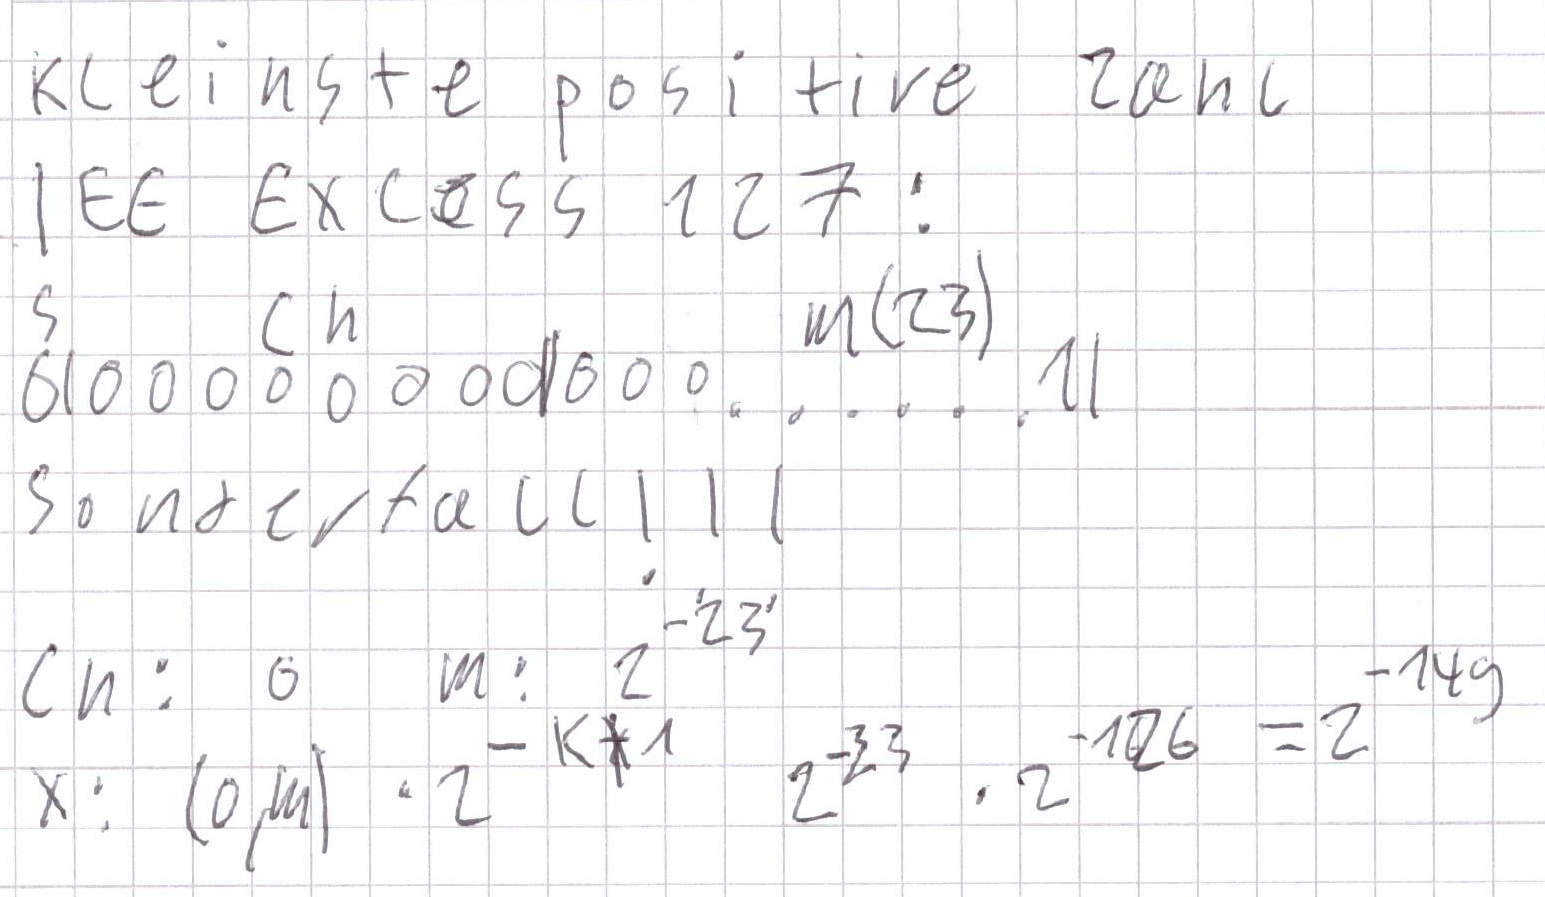
\includegraphics[width=\linewidth]{102b}
	\subsection*{c)}
	Die Mantisse besitzt 23 Stellen. Um alle Kommazahlen zu erschlagen muss das Komma um 23 Stellen nach rechts verschoben werden. Daraus folgt, dass ab dem Exponenten 23 keine Kommazahlen mehr darstellbar sind. \\
	Bei Exponent 23 ist der Abstand zwischen zwei Zahlen 1 und bei 24 zwei. Daraus ergibt sich der Zahlenbereich von $2^{23} \to 2^{24}$.
	\section*{Aufgabe 10.3}
	\subsection*{a)}
	0A = LF; 62 = b; 61 = a;  \\
	a LF b LF \\
	a \\
	b \\
	\subsection*{b)}
	Aus historischen Gründen: Bei einer Schreibmaschine muss das Blatt erst nach oben geschoben werden bevor eine neue Zeile begonnen werden kann. MS Dos war seiner Zeit diesem Prinzip nachempfunden.
	\subsection*{c)}
	@ $\to$ basic latin u+0040 \\
	x $\to$ basic latin u+0078 \\
	Ö $\to$ latin-1 Supplement u+00D6 \\
	$\infty$ $\to$ mathmetical operators u+221E \\
	smiley $\to$ U+263A \\
	halbe Note $\to$ u+1D15E
	\subsection*{d)}
	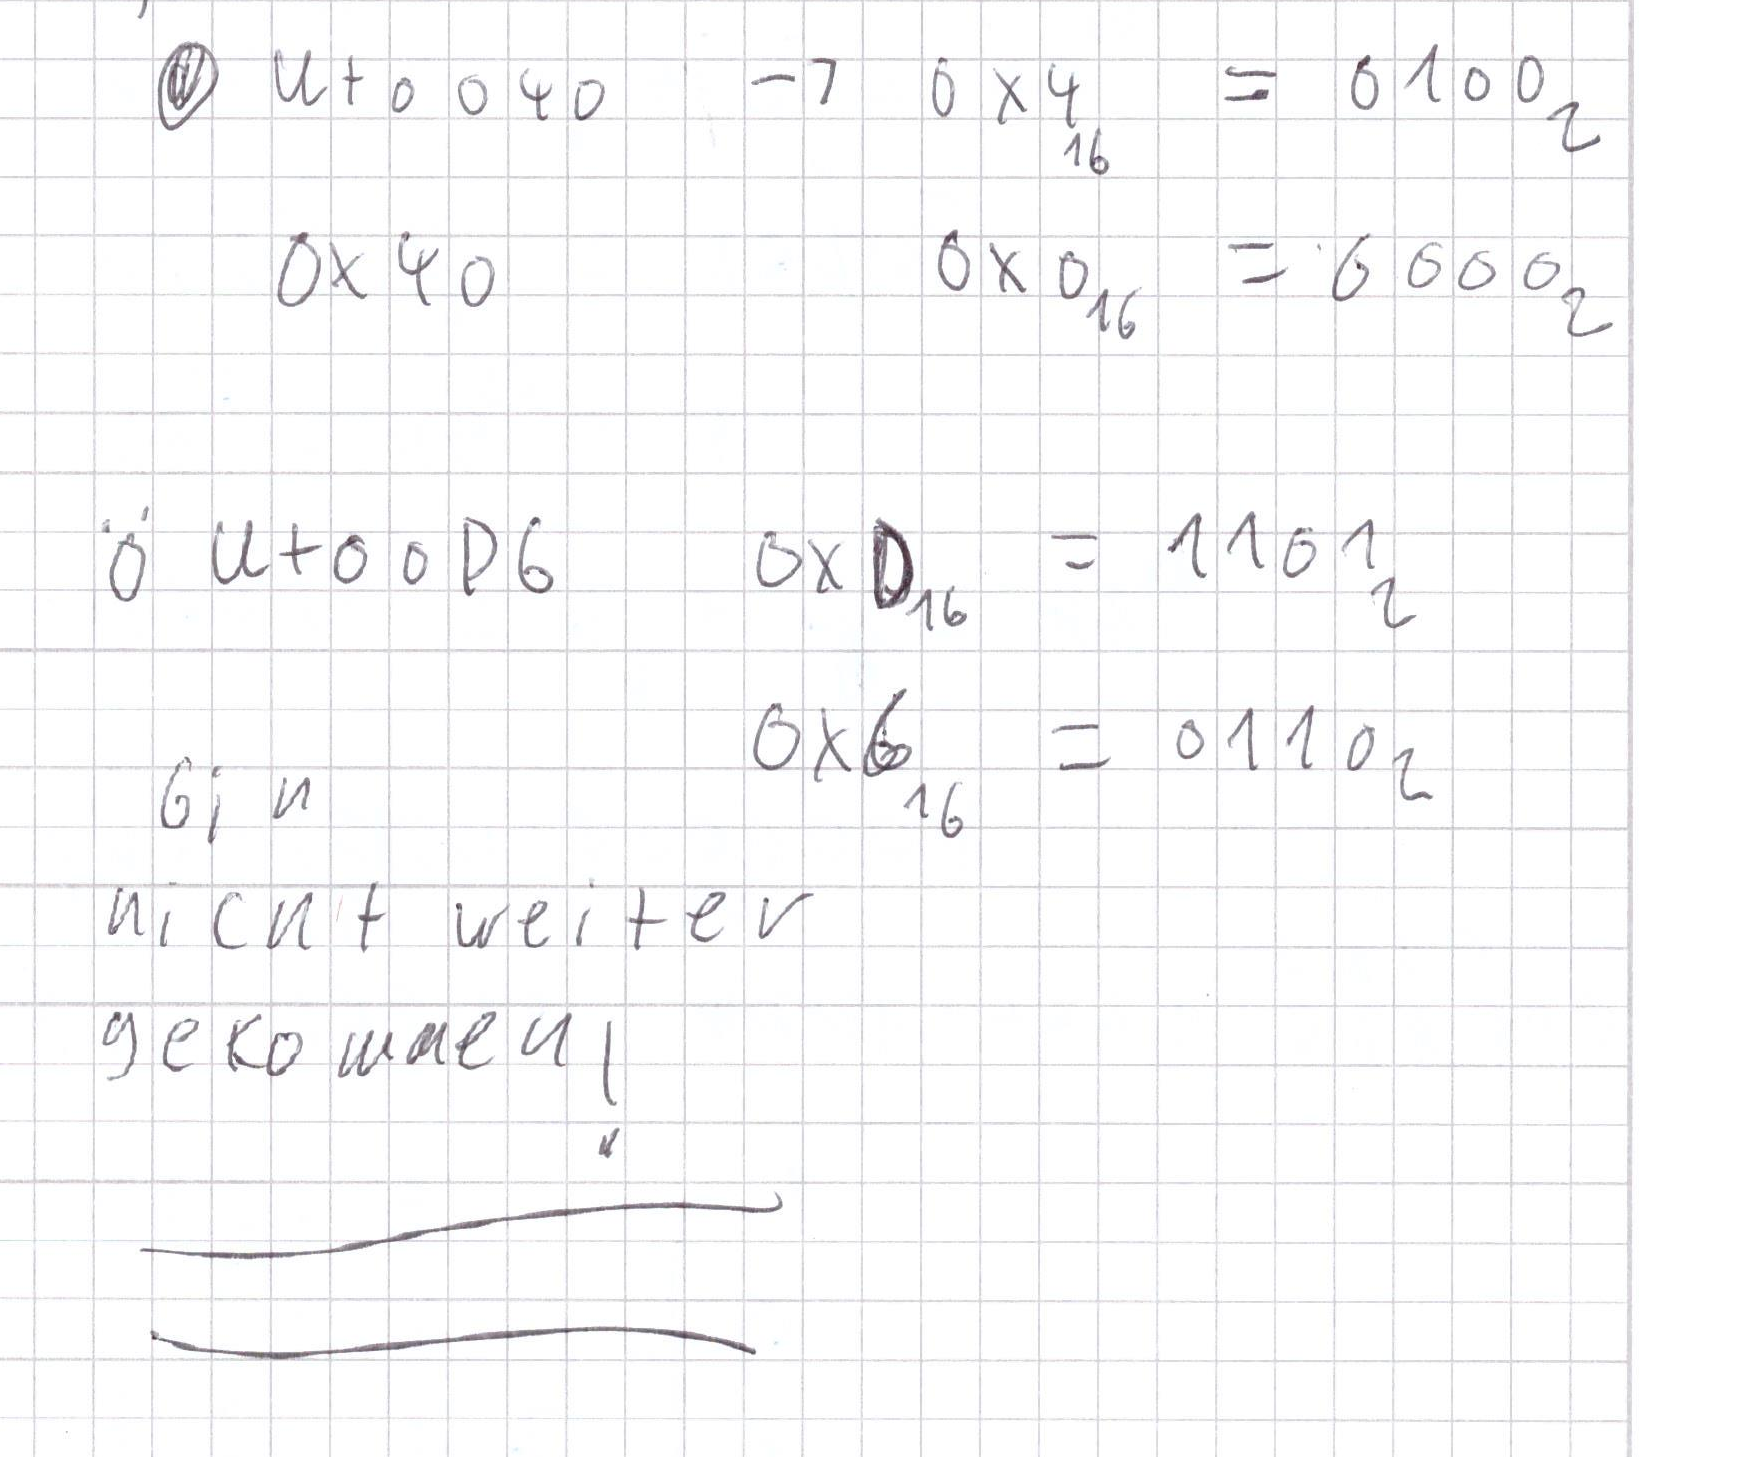
\includegraphics[width=\linewidth]{103d}
	\section*{Aufgabe 10.4}
	Es handelt sich um ein Muster bei dem immer 8 Ziffern zur Basis zwei hintereinander stehen. Vermutung legt ASCII-Code nahe.\\ \\
	\begin{tabular}[h]{c|c|c}
		Binärmuster & Hex-Darstellung & ASCII-Zeichen \\
		\hline \\
		00100010 & 0x22 & " \\
		01001001 & 0x49 & I \\ 
	\end{tabular} \\
	Aus Zeitgründen ist die Lösung hier nur angedeutet. Die Lösung eines Kommilitonen ergibt: "Informatik in gesellschaftlicher Verantwortung".
	\section*{Aufgabe 10.5}
	\subsection*{a)}
	Es wird 44100 mal je Sekunde auf zwei Kanälen je eine 16-Bit Zahl gelesen. \\
	Daraus Folgt: 44,1 kHz * 16 bit * 2 Stereo-Kanäle * Zeit in Sekunden \\ \\
	1 Std = 60 min = 3600 Sekunden \\
	44100 * 16 * 2 = 1.411.200 bit/s \\
	$\frac{1.411.200}{8} = 176400 Byte/s$ \\ \\
	Für eine einstündige Musikaufnahme folgt daraus wiederum: \\ \\
	44100 * 16 * 2 * 3600 = 5080320000 bit \\
	5.080.320.000 bit = 635.040.000 byte \\
	$\frac{635.040.000 byte}{1024*1024} \approx 606 Mebibyte$
	\subsection*{b)}
	Größte zahl für 8-Bit AD-Wandler: $11111111_2 = 255_{10}$ \\
	\includegraphics[width=\linewidth]{"105b"} \\
	Daraus ergibt sich maximaler Dynamikumfang für einen 8-Bit AD-Wandler: \\ \\
	$L_p = 20 * log_{10}(255/1)$ \\
	$L_p \approx 48,13 dB$ \\ \\
	größte Zahl 16-Bit AD-Wandler: \\
	$1111111111111111_2 = 65535_{10}$ \\
	$L_p = 20 * log_{10}(65535/1)$ \\
	$L_p \approx 96,33 dB$ \\ \\
	Der maximale Dynamikumfang einer Audio-CD beträgt $\approx$ 96,33 dB. Mit einem 8-Bit AD-Wandler erhält man jedoch lediglich  $\approx$ 48,13 dB.
	\subsection*{c)}
	Aus Zeitgründen entfallen.
	\section*{Aufgabe 10.6}
	\subsection*{a)}
	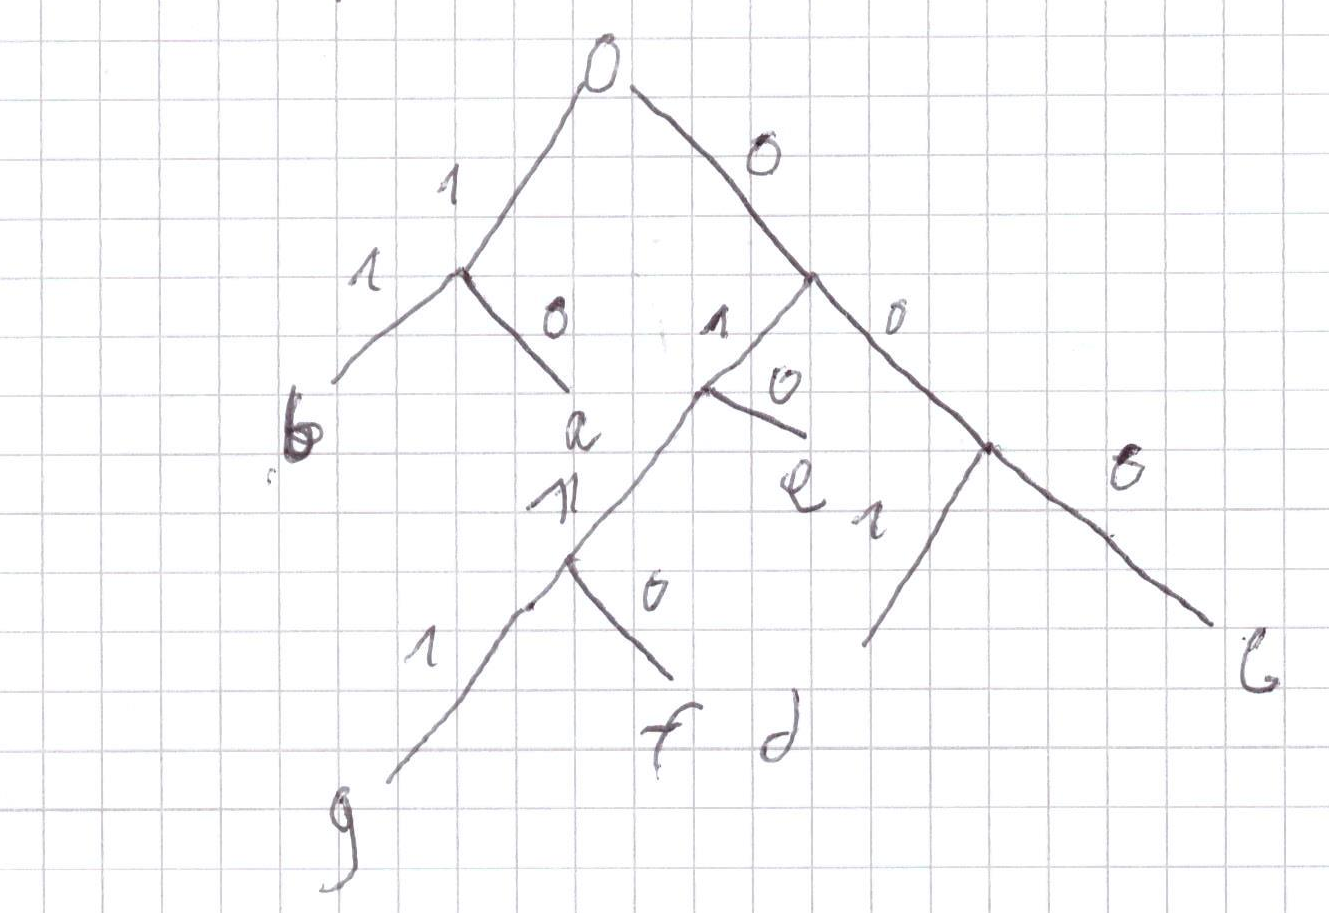
\includegraphics[width=\linewidth]{106a}
	\subsection*{b)}
	Kein Codewort ist Präfix eines anderen Codewortes. Die Farno-Bedingung ist damit erfüllt.
	\subsection*{c)}
	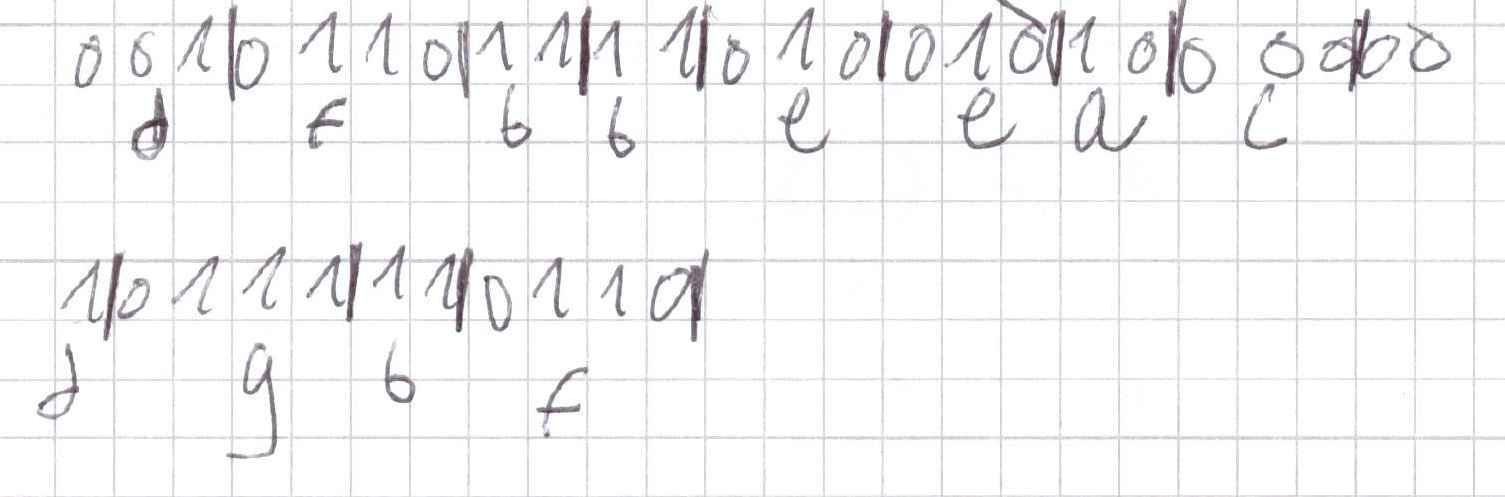
\includegraphics[width=\linewidth]{106c}
\end{document}